%% ch03-qgear.tex — Chapter III: GPU-Accelerated Circuit Simulation at HPC Scale (Q-GEAR)
\chapter{GPU-Accelerated Circuit Simulation at HPC Scale}\label{ch:qgear}

\authorshipstatement{This chapter is based on Z.~Guo, J.~Balewski and Z.~Pan, ``Q-GEAR: Improving quantum simulation framework,'' published in the Proceedings of the 54th International Conference on Parallel Processing (ACM ICPP~2025) \cite{guo2025qgear}, and on the accompanying open-source software release \cite{guo2025qgearsoftware}. The candidate designed the framework, implemented the circuit encoder, the kernel transformation and the container images, ran all CPU and GPU experiments on the NERSC Perlmutter system and the TTU High Performance Computing Center, and wrote the manuscript. J.~Balewski advised on the HPC deployment, the multi-node CUDA-Q configuration and the QCrank benchmarks; Z.~Pan supervised the work. The work was supported by the U.S.\ Department of Energy, Office of Science, through NERSC award DDR-ERCAP0034486.}

This chapter addresses RQ1: how far classical high-performance computing can push exact state-vector simulation of quantum circuits, and how that capability can be made usable by researchers who already have a large body of \qiskit\ programs and cannot afford to rewrite them for every new accelerator back end. We present \qgear, a framework that encodes \qiskit\ circuits into a small set of dense tensors, translates them gate by gate into \cudaq\ kernels, and packages the whole stack as Slurm-ready container images for multi-GPU, multi-node execution. We report experiments from \cite{guo2025qgear} in which random unitary circuits of up to 42 qubits were simulated on up to 1,024 NVIDIA A100 GPUs, a 34-qubit circuit that required roughly one day on a 128-core CPU node finished in about one minute on four GPUs, and the same pipeline delivered order-of-magnitude gains over existing GPU simulators for the Quantum Fourier transform and for \qcrank\ image-encoding circuits. The chapter closes by discussing the memory wall that bounds exact simulation and by describing how \qgear\ serves as the simulation substrate for the remaining research chapters of this dissertation.

\section{Introduction and Motivation}\label{sec:qgear:intro}

Classical simulation is the indispensable companion of every quantum-computing research program. Before a circuit is submitted to a quantum processing unit (QPU), it is simulated to check that the algorithm is correct, to calibrate hyper-parameters, to estimate the shot budget, and to predict which features of the output distribution should survive hardware noise. After the hardware run, simulation provides the noiseless reference against which fidelity, energy error and success probability are measured. The difficulty is that exact state-vector simulation of an $n$-qubit circuit stores $2^{n}$ complex amplitudes and touches all of them for every gate, so both memory and time grow exponentially in $n$ (\cref{sec:bg:sim}). At $n=34$ a single-precision state vector occupies \SI{128}{\giga\byte}; at $n=42$ it occupies \SI{32}{\tera\byte}. This exponential ``simulation wall'' is precisely what makes quantum computers interesting \cite{arute2019supremacy,preskill2018nisq}, but it is also what makes it difficult to develop, verify and calibrate circuits in the 30--45-qubit regime that current superconducting and trapped-ion processors can execute.

Graphics processing units (GPUs) are the natural instrument for pushing back this wall. A state-vector update is a memory-bound, embarrassingly data-parallel operation that maps well to the thousands of streaming cores and the \SI{1.5}{\tera\byte\per\second} memory bandwidth of an NVIDIA A100 \cite{choquette2021a100}. NVIDIA's cuQuantum library \cite{bayraktar2023cuquantum} and the \cudaq\ programming model built on it \cite{kim2023cudaquantum} expose this hardware through kernels that can be distributed across many GPUs with the Message Passing Interface (MPI), and several research simulators have demonstrated single-GPU state-vector performance far beyond that of CPU back ends \cite{suzuki2021qulacs,vanbeeumen2023qclabpp,doi2023multishotgpu,asadi2024pennylanelightning}. Yet the community's circuits are overwhelmingly written in \qiskit\ \cite{javadiabhari2024qiskit}, whose ecosystem of transpilers, hardware providers and algorithm libraries has no counterpart in the GPU-native toolchains. In our experience, and in the experience of the collaborators whose circuits motivated this work, a researcher who wants GPU performance faces a choice between two unattractive options: rewrite the circuit in a new domain-specific language, learning its idioms and re-validating every gate, or accept the CPU back end and its multi-hour turnaround.

\qgear\ removes this choice. Its premise is that a researcher should not have to rewrite a circuit to change the machine that simulates it. The framework accepts an ordinary \qiskit\ \texttt{QuantumCircuit}, serialises it into three pre-allocated tensors, and re-materialises it as a \cudaq\ kernel whose cost is constant per gate, so that the translation itself is negligible next to the simulation. The kernel is then executed on whatever target is available: a single GPU, the four GPUs of a Perlmutter node, or hundreds of nodes connected by the Slingshot interconnect. The entire software stack, from Python and \qiskit\ to \cudaq, MPI and the CUDA driver interface, is captured in a Podman-HPC/Shifter container image so that the deployment is reproducible and independent of the modules installed on the host. In summary, this chapter makes the following contributions, all reported in \cite{guo2025qgear} and released as open-source software \cite{guo2025qgearsoftware}.
\begin{enumerate}
  \item A compact tensor encoding of batches of quantum circuits, together with an HDF5-based storage layout with JSON metadata, that decouples circuit generation from circuit execution and allows thousands of circuits to be shipped between CPU and GPU nodes as a single file (\cref{sec:qgear:encoding}).
  \item A gate-by-gate transformation from \qiskit\ gate objects to \cudaq\ kernel instructions in constant time per gate, currently covering the gate set H, RY, RZ, U3, CX, CP, SWAP and measurement (\cref{sec:qgear:kernel}).
  \item Two execution modes, an \emph{adjoint} mode that composes many sub-circuits or Hamiltonian terms into one large state-vector simulation, and a \emph{parallel} mode that dispatches independent circuits to independent GPUs (\cref{sec:qgear:modes}).
  \item A containerised, Slurm-integrated deployment on NERSC Perlmutter that uses \cudaq's \texttt{nvidia-mgpu} target to partition a single state vector across up to 1,024 A100 GPUs by index-bit decomposition (\cref{sec:qgear:deploy}).
  \item An experimental evaluation on random unitary circuits, the Quantum Fourier transform (QFT), a variational quantum eigensolver (VQE) and \qcrank\ image-encoding circuits, showing roughly two orders of magnitude speed-up over a 128-core CPU node, roughly one order of magnitude over existing GPU simulators, and strong scaling to 42 qubits (\cref{sec:qgear:results}).
\end{enumerate}

\section{Problem Statement and Preliminaries}\label{sec:qgear:problem}

The mathematical background of state-vector simulation is given in \cref{sec:bg:sim}; here we fix only the notation and the cost model that the design of \qgear\ responds to. An $n$-qubit pure state is a vector $\ket{\psi}\in\C^{2^{n}}$ with amplitudes $\psi_{i}$ indexed by the bit string $i=(i_{n-1}\cdots i_{1}i_{0})_{2}$, where bit $i_{q}$ is the computational-basis value of qubit $q$. A single-qubit gate $U$ on qubit $q$ updates every pair of amplitudes whose indices differ only in bit $q$,
\begin{equation}\label{eq:qgear:sqgate}
  \begin{pmatrix}\psi'_{i\,[i_{q}=0]}\\ \psi'_{i\,[i_{q}=1]}\end{pmatrix}
  = U \begin{pmatrix}\psi_{i\,[i_{q}=0]}\\ \psi_{i\,[i_{q}=1]}\end{pmatrix},
  \qquad \text{for all } 2^{n-1} \text{ such pairs},
\end{equation}
and a two-qubit gate acts analogously on quadruples of amplitudes. Every gate therefore performs $\Theta(2^{n})$ arithmetic operations and, more importantly, streams the whole state vector through memory. For a circuit with $m$ gates the time is $\Theta(m\,2^{n})$ and the memory is $2^{n}\times 8$ bytes in single precision (complex64) or $2^{n}\times 16$ bytes in double precision. The 128-core CPU node used as our baseline has \SI{512}{\giga\byte} of DRAM and a few hundred gigabytes per second of aggregate memory bandwidth, so a 34-qubit single-precision state (\SI{128}{\giga\byte}) can be held but each gate costs on the order of a second; a circuit with $10^{4}$ two-qubit gates then runs for hours. A single A100 with \SI{40}{\giga\byte} of high-bandwidth memory holds a 32-qubit single-precision state (\SI{32}{\giga\byte}) and streams it in tens of milliseconds, so the same circuit finishes in seconds, but adding one qubit requires doubling the memory, that is, doubling the number of GPUs.

From this cost model we derive the four requirements that \qgear\ must meet. First, \emph{transparency}: the input is a \qiskit\ circuit and the user never writes \cudaq\ code. Second, \emph{negligible translation cost}: the translation from \qiskit\ to \cudaq\ must be $\bigO{m}$ with a small constant so that it is invisible next to the $\Theta(m 2^{n})$ simulation. Third, \emph{scalability}: the same pipeline must run on one GPU, on the four GPUs of a node and on hundreds of nodes, using the memory of all GPUs for a single state vector when the circuit is too large for one device. Fourth, \emph{reproducibility}: the software stack must be captured in a container and driven by ordinary Slurm batch scripts so that an experiment can be repeated on a different allocation or a different HPC centre.

\section{Design of \qgear}\label{sec:qgear:design}

\Cref{fig:qgear:pipeline} gives an overview of the \qgear\ pipeline. A batch of \qiskit\ circuits is encoded once into three tensors and written, together with JSON metadata, to an HDF5 file; the file is read by a kernel builder that emits one \cudaq\ kernel per circuit; and the kernels are executed on the selected GPU target, returning state vectors, measurement counts or observable expectation values. The following subsections describe each stage.

% alt: Block diagram of the Q-GEAR pipeline. Top row: a Qiskit QuantumCircuit enters an encoder that produces three tensors (circ_type, gate_type, gate_param) which are stored in an HDF5 file with JSON metadata. Bottom row: the HDF5 file is read by a kernel builder that emits a CUDA-Q kernel, which runs on the nvidia or nvidia-mgpu target and returns results.
\begin{figure}[htbp]
\centering
\begin{tikzpicture}[
  font=\footnotesize,
  box/.style={draw,rounded corners=2pt,align=center,minimum height=9mm,inner sep=2pt,text width=26mm},
  tens/.style={draw,fill=cbSky!20,align=center,minimum height=7mm,inner sep=2pt,text width=29mm,font=\footnotesize\ttfamily},
  arr/.style={-{Latex[length=2mm]},thick}]
  % top row
  \node[box,fill=cbGray!10,text width=30mm] (qc) at (0,0) {\qiskit\\ \texttt{QuantumCircuit}\\ (H, RY, RZ, U3,\\ CX, CP, SWAP, M)};
  \node[box] (enc) at (4.0,0) {Encoder\\ one pass over the\\ gate list};
  \node[tens] (t1) at (8.4,1.55) {circ\_type\\ (nCirc,2)\\ int32};
  \node[tens] (t2) at (8.4,0) {gate\_type\\ (nCirc,nGate,3)\\ int32};
  \node[tens] (t3) at (8.4,-1.55) {gate\_param\\ (nCirc,nGate,3)\\ float32};
  \node[box,fill=cbOrange!15] (h5) at (12.4,0) {HDF5 file\\ + JSON metadata};
  \draw[arr] (qc) -- (enc);
  \draw[arr] (enc.east) -- (t1.west);
  \draw[arr] (enc.east) -- (t2.west);
  \draw[arr] (enc.east) -- (t3.west);
  \draw[arr] (t1.east) -- (h5.west);
  \draw[arr] (t2.east) -- (h5.west);
  \draw[arr] (t3.east) -- (h5.west);
  % bottom row
  \node[box] (kb) at (12.4,-3.5) {Kernel builder\\ $\bigO{1}$ per gate};
  \node[box,fill=cbGreen!15] (ker) at (8.4,-3.5) {\cudaq\ kernel\\ (\texttt{h}, \texttt{ry}, \texttt{rz}, \texttt{u3},\\ \texttt{cx}, \texttt{cr1}, \texttt{swap}, \texttt{mz})};
  \node[box] (tgt) at (4.0,-3.5) {Target\\ \texttt{nvidia} (1 GPU)\\ \texttt{nvidia-mgpu} (MPI)};
  \node[box,fill=cbGray!10,text width=30mm] (out) at (0,-3.5) {Results\\ state vector,\\ counts, $\expval{H}$};
  \draw[arr] (h5) -- (kb);
  \draw[arr] (kb) -- (ker);
  \draw[arr] (ker) -- (tgt);
  \draw[arr] (tgt) -- (out);
  % mode annotations
  \node[align=left,font=\scriptsize,anchor=north] at (4.0,-4.45) {adjoint mode: $H_{1}+\dots+H_{N}$ on one state\\ parallel mode: circuit$_{1},\dots,$circuit$_{N}$ on $N$ ranks};
\end{tikzpicture}
\caption{The \qgear\ pipeline. A batch of \qiskit\ circuits is encoded once into three dense tensors and stored as HDF5 with JSON metadata; a kernel builder re-materialises each circuit as a \cudaq\ kernel in constant time per gate and executes it on a single-GPU or multi-GPU target. Schematic.}
\label{fig:qgear:pipeline}
\end{figure}

\subsection{Circuit Encoding into Pre-Allocated Tensors}\label{sec:qgear:encoding}

The first design decision is to separate the \emph{generation} of circuits, which is typically done in \qiskit\ on a CPU login node or in a Jupyter session, from their \emph{execution}, which happens on GPU compute nodes reached through the batch scheduler. Serialising \qiskit\ circuit objects directly, for example with OpenQASM text or Python pickles, is possible but slow to parse and awkward to distribute over MPI ranks. \qgear\ instead encodes a batch of $N_{\mathrm{circ}}$ circuits, each with at most $N_{\mathrm{gate}}$ gates, into three pre-allocated arrays whose shapes are known before the first gate is visited:
\begin{itemize}
  \item \texttt{circ\_type} of shape $(N_{\mathrm{circ}},2)$ and type \texttt{int32}, holding for each circuit the pair $[\texttt{num\_qubit},\texttt{num\_gate}]$;
  \item \texttt{gate\_type} of shape $(N_{\mathrm{circ}},N_{\mathrm{gate}},3)$ and type \texttt{int32}, holding for each gate the triple $[\texttt{gate\_type},\texttt{qubit1},\texttt{qubit2}]$, where \texttt{gate\_type} is an integer code from the dictionary in \cref{tab:qgear:gates} and \texttt{qubit2} is set to $-1$ for single-qubit gates;
  \item \texttt{gate\_param} of shape $(N_{\mathrm{circ}},N_{\mathrm{gate}},3)$ and type \texttt{float32}, holding up to three real parameters per gate, namely $(\theta,\phi,\lambda)$ for U3, $(\theta,0,0)$ for RY, RZ and CP, and zeros for parameter-free gates.
\end{itemize}
Circuits shorter than $N_{\mathrm{gate}}$ are padded with a reserved no-operation code so that all rows have the same length, and the padding is skipped by the kernel builder using the \texttt{num\_gate} entry of \texttt{circ\_type}. The encoder makes a single pass over the \qiskit\ gate list, so the encoding cost is $\bigO{N_{\mathrm{circ}}N_{\mathrm{gate}}}$ with a constant dominated by attribute look-ups on the \qiskit\ objects; for the largest batches used in \cite{guo2025qgear}, with $10^{4}$ two-qubit gates per circuit, encoding takes a fraction of a second and is amortised over every subsequent execution of the batch.

The three tensors are written to an HDF5 file with the same three dataset names, and a JSON document stored as an HDF5 attribute records the metadata needed to interpret them: the gate dictionary, the qubit counts, the random seed or image identifier that generated the batch, the \qiskit\ version and a time stamp. HDF5 was chosen because it is the lingua franca of HPC data management, is readable from every language in the stack, supports parallel I/O from many MPI ranks, and stores dense typed arrays without the parsing overhead of text formats. The encoded batch is thus a self-describing artefact: it can be regenerated deterministically, shipped to another machine, inspected with standard tools, and executed on any \cudaq\ target without access to the code that produced it. The appendix material of \cite{guo2025qgear} and the software repository \cite{guo2025qgearsoftware} document the exact layout; \cref{app:qgear} reproduces the dataset names and the metadata schema.

The supported gate set and its mapping onto \cudaq\ primitives is summarised in \cref{tab:qgear:gates}. The set is deliberately small. Together with the \qiskit\ transpiler, which can rewrite any circuit into $\{$U3, CX$\}$, it is universal, and the additional native entries for H, RY, RZ, CP and SWAP avoid the gate-count inflation that a full decomposition would cause for the QFT and \qcrank\ workloads that motivated the framework. Gates outside the set are rejected with a message that names the offending instruction and suggests the transpiler basis to use.

\begin{table}[htbp]
\caption{Gate-set coverage of \qgear\ and the mapping from \qiskit\ instructions to \cudaq\ kernel primitives. The integer code is stored in \texttt{gate\_type}; the parameter slots refer to \texttt{gate\_param}. From \cite{guo2025qgear,guo2025qgearsoftware}.}
\label{tab:qgear:gates}
\centering\small
\begin{threeparttable}
\begin{tabular}{@{}lllccl@{}}
\toprule
\qiskit\ gate & \cudaq\ primitive & Matrix / action & Qubits & Params & Notes \\
\midrule
\texttt{h}       & \texttt{h(q)}                    & Hadamard                          & 1 & 0 & Clifford \\
\texttt{ry}      & \texttt{ry(\(\theta\),q)}        & $e^{-i\theta Y/2}$                & 1 & 1 & \qcrank\ data rotations \\
\texttt{rz}      & \texttt{rz(\(\theta\),q)}        & $e^{-i\theta Z/2}$                & 1 & 1 & virtual on hardware \\
\texttt{u3}      & \texttt{u3(\(\theta,\phi,\lambda\),q)} & general $SU(2)$             & 1 & 3 & random unitaries \\
\texttt{cx}      & \texttt{cx(c,t)}                 & controlled-$X$                    & 2 & 0 & entangler \\
\texttt{cp}      & \texttt{cr1(\(\theta\),c,t)}     & $\mathrm{diag}(1,1,1,e^{i\theta})$ & 2 & 1 & QFT phases\tnote{a} \\
\texttt{swap}    & \texttt{swap(a,b)}               & exchange                          & 2 & 0 & QFT bit reversal \\
\texttt{measure} & \texttt{mz(q)}                   & $Z$-basis readout                 & 1 & 0 & to classical register \\
\bottomrule
\end{tabular}
\begin{tablenotes}\footnotesize
\item[a] \qiskit's \texttt{cp} and \cudaq's controlled \texttt{r1} share the same matrix, so no phase correction is needed.
\end{tablenotes}
\end{threeparttable}
\end{table}

\subsection{Gate-by-Gate Kernel Transformation}\label{sec:qgear:kernel}

The kernel builder reads one row of \texttt{circ\_type}, allocates a \cudaq\ qubit register of the recorded size, and then iterates over the first \texttt{num\_gate} rows of \texttt{gate\_type}, dispatching each integer code to the corresponding kernel primitive with the qubit indices and parameters read from the same row of \texttt{gate\_type} and \texttt{gate\_param}. Because the dispatch is a table look-up and the primitive call appends one instruction to the kernel, the work per gate is constant and independent of $n$; the total translation time is $\bigO{m}$ for an $m$-gate circuit. The resulting kernel is a genuine \cudaq\ program: it is compiled once by the \cudaq\ just-in-time pipeline into the intermediate representation consumed by the target, and it can be executed with \texttt{cudaq.sample} to obtain counts, with \texttt{cudaq.observe} to obtain expectation values of a spin operator, or with \texttt{cudaq.get\_state} to retrieve the full state vector for fidelity checks against the \qiskit\ reference on small instances.

Two properties of this construction are worth emphasising. First, it is \emph{lossless} for the supported gate set: every gate is mapped to a primitive with exactly the same unitary, so a circuit simulated through \qgear\ produces, up to floating-point rounding, the same state vector as the \qiskit\ Aer simulator on the original circuit. This was verified in \cite{guo2025qgear} on small instances by comparing state vectors and on the VQE benchmark by comparing converged energies (\cref{sec:qgear:results-comparison}). Second, the construction is \emph{stateless}: the builder does not need the original \qiskit\ objects, only the tensors, which is what allows the encoding to be done on a login node and the kernel construction to be done independently on every MPI rank of a large job, without pickling Python objects across processes.

\subsection{Workflow Modes: Adjoint and Parallel}\label{sec:qgear:modes}

Quantum-computing workloads on an HPC system come in two shapes, and \qgear\ exposes one execution mode for each. In \emph{adjoint mode} a single large computation is assembled from many pieces: for instance the cost Hamiltonian of a variational algorithm is a sum $H=H_{1}+\dots+H_{N}$ of Pauli terms, or a long circuit is the concatenation of many sub-circuits generated independently. \qgear\ then composes the pieces into one kernel and one spin operator and executes them as a single state-vector simulation, so that all $N$ expectation values $\expval{H_{k}}$ are read from one state and, when gradients are needed, are obtained by adjoint differentiation \cite{jones2020adjoint} in a single backward sweep rather than by $2N$ parameter-shift evaluations. This mode is the one that benefits from the multi-GPU state-vector partitioning of \cref{sec:qgear:deploy}, because the state is large and shared. In \emph{parallel mode} the workload consists of $N$ independent circuits, such as the batch of random circuits used for benchmarking, the many \qcrank\ sub-images of a large picture, or the population of candidate circuits produced by a synthesis loop (\cref{ch:synthesis}). Each MPI rank then reads its slice of the HDF5 batch, builds its own kernels, and simulates them on its own GPU with the single-device \texttt{nvidia} target; there is no inter-rank communication apart from the final gather of results. Both modes are selected by a single command-line flag in the Slurm script and share the encoder, the kernel builder and the container image.

\subsection{Containerised Deployment and Multi-GPU Execution}\label{sec:qgear:deploy}

Reproducible deployment on a shared HPC system is a software-engineering problem as much as a performance problem. The \cudaq\ tool-chain depends on a specific CUDA driver interface, a specific MPI implementation, and a Python environment that must match the \qiskit\ version used to generate the circuits. \qgear\ freezes this stack in an Open Container Initiative image derived from the official \cudaq\ image, with \qiskit, h5py and the \qgear\ package added, and runs it through Podman-HPC on Perlmutter \cite{stephey2022podman} (Shifter images are produced from the same definition for systems that do not support Podman-HPC). The image is launched by Slurm with one task per GPU; the Slurm plugin exposes the Cray MPICH libraries of the host to the container so that the containerised \cudaq\ runtime can use the Slingshot interconnect directly rather than falling back to TCP. A typical job script requests $R$ GPU nodes, sets the \cudaq\ target to \texttt{nvidia-mgpu}, and launches $4R$ ranks with \texttt{srun}; the same script with the target set to \texttt{nvidia} runs the parallel mode. The Slurm scripts, image definitions and environment files are part of the released software \cite{guo2025qgearsoftware} and are listed in \cref{app:qgear}.

The \texttt{nvidia-mgpu} target distributes one state vector over $G=2^{g}$ GPUs by \emph{index-bit partitioning}, illustrated in \cref{fig:qgear:partition}. Write the amplitude index as $i=(i_{n-1}\cdots i_{0})_{2}$. The $g$ most significant bits $(i_{n-1}\cdots i_{n-g})$ are interpreted as the rank of the GPU that owns the amplitude, and the remaining $n-g$ bits are the offset of the amplitude inside that GPU's local array of $2^{n-g}$ elements. Each GPU therefore stores a contiguous block of $2^{n-g}$ amplitudes, and the memory requirement per GPU is $2^{n-g}\times 8$ bytes in single precision. On A100 GPUs with \SI{40}{\giga\byte} this bounds the local block to $2^{32}$ amplitudes, so $G$ GPUs can hold at most $n = 32+g$ qubits: 32 qubits on one GPU, 34 on the four GPUs of a node, 36 on four nodes, and 42 on $2^{10}=1,024$ GPUs, which is exactly the largest configuration reported in \cite{guo2025qgear}. Qubits $0,\dots,n-g-1$ are called \emph{local} and qubits $n-g,\dots,n-1$ are called \emph{global}.

The partition determines which gates need communication. A single-qubit gate on a local qubit $q<n-g$ pairs amplitudes whose indices differ in bit $q$; both amplitudes of each pair have the same top $g$ bits and therefore live on the same GPU, so the update in \cref{eq:qgear:sqgate} is entirely local and all $G$ GPUs proceed in parallel with no data movement. A single-qubit gate on a global qubit $q\geq n-g$ pairs amplitudes whose GPU ranks differ in bit $q-(n-g)$: every GPU must exchange half of its block, $2^{n-g-1}$ amplitudes, with its partner GPU before the update can be applied. \cudaq\ implements this as a pairwise exchange over NVLink within a node and over the Slingshot network between nodes, or, when several global gates follow one another, as a permutation of the qubit ordering that turns global qubits into local ones and back. Two-qubit gates follow the same rule for each of their qubits, with one important simplification for controlled gates: if only the \emph{control} qubit is global, no amplitudes need to be exchanged, because the gate acts as the identity on the GPUs whose rank bit is 0 and as the target operation on those whose rank bit is 1, so each GPU simply either applies the local update or does nothing. Only a global \emph{target} qubit forces communication. The communication volume per global gate is $2^{n-g-1}\times 8$ bytes per GPU, which for a 42-qubit state on 1,024 GPUs is \SI{16}{\giga\byte} per GPU and per gate; the fact that the measured GPU utilisation nevertheless stayed near 100\% (\cref{sec:qgear:results-scaling}) reflects both the high bandwidth of NVLink and Slingshot and the fact that only the $g$ global qubits, a small minority of the $n$ qubits in a random circuit, ever trigger an exchange.

% alt: Schematic of index-bit partitioning of a 2^n state vector across four GPUs. A horizontal strip of amplitudes is divided into four colored blocks labelled GPU 0 to GPU 3 by the two most significant index bits. Below, the index bit field is split into a GPU-rank part (g bits) and a local-offset part (n-g bits). A short double arrow inside one block shows that a gate on a local qubit pairs amplitudes within a GPU; a long arc between GPU 0 and GPU 2 shows that a gate on a global qubit pairs amplitudes on different GPUs and requires communication.
\begin{figure}[htbp]
\centering
\begin{tikzpicture}[font=\footnotesize, arr/.style={{Latex[length=1.6mm]}-{Latex[length=1.6mm]},thick}]
  % amplitude strip split over G = 4 GPUs
  \foreach \g/\c/\b in {0/cbBlue/00, 1/cbOrange/01, 2/cbGreen/10, 3/cbRed/11} {
    \draw[fill=\c!20,draw=\c,thick] (\g*3.3,0) rectangle ++(3.3,0.9);
    \node at (\g*3.3+1.65,0.62) {GPU \g};
    \node[font=\scriptsize] at (\g*3.3+1.65,0.25) {$i_{n-1}i_{n-2}=\b$, $2^{n-2}$ ampl.};
  }
  \node[anchor=south west,font=\footnotesize] at (9.6,1.05) {$\ket{\psi}\in\C^{2^{n}}$, $G=4$ GPUs};
  % local gate arrow inside GPU 0
  \draw[arr,cbBlue] (0.5,1.05) to[bend left=50] (1.5,1.05);
  \node[font=\scriptsize,cbBlue,anchor=south west] at (0.0,1.35) {local qubit $q<n-g$: both amplitudes on one GPU};
  % global gate arrow between GPU 0 and GPU 2
  \draw[arr,cbRed] (2.4,-0.15) to[bend right=25] (7.4,-0.15);
  \node[font=\scriptsize,cbRed,anchor=north] at (5.0,-0.85) {global qubit $q=n-1$: partner on another GPU (exchange $2^{n-g-1}$ amplitudes)};
  % bit field
  \begin{scope}[yshift=-2.5cm]
    \draw[thick] (1.8,0) rectangle ++(1.3,0.7); \node at (2.45,0.35) {$i_{n-1}$};
    \draw[thick] (3.1,0) rectangle ++(1.3,0.7); \node at (3.75,0.35) {$i_{n-2}$};
    \draw[thick] (4.4,0) rectangle ++(1.3,0.7); \node at (5.05,0.35) {$i_{n-3}$};
    \draw[thick] (5.7,0) rectangle ++(3.6,0.7); \node at (7.5,0.35) {$\cdots$};
    \draw[thick] (9.3,0) rectangle ++(1.3,0.7); \node at (9.95,0.35) {$i_{1}$};
    \draw[thick] (10.6,0) rectangle ++(1.3,0.7); \node at (11.25,0.35) {$i_{0}$};
    \draw[decorate,decoration={brace,mirror,amplitude=5pt}] (1.8,-0.1) -- (4.4,-0.1) node[midway,below=6pt] {GPU rank ($g=2$ bits)};
    \draw[decorate,decoration={brace,mirror,amplitude=5pt}] (4.4,-0.1) -- (11.9,-0.1) node[midway,below=6pt] {local offset ($n-g$ bits)};
    \node[anchor=east] at (1.6,0.35) {index $i$:};
  \end{scope}
\end{tikzpicture}
\caption{Index-bit partitioning of a $2^{n}$-amplitude state vector over $G=2^{g}$ GPUs (here $G=4$). The $g$ most significant index bits select the GPU and the remaining $n-g$ bits address the amplitude inside the GPU's block. Gates on local qubits need no communication; gates whose target is a global qubit require each GPU to exchange half of its block with a partner. Schematic.}
\label{fig:qgear:partition}
\end{figure}

\section{Implementation}\label{sec:qgear:impl}

\qgear\ is implemented as a Python package developed with the nbdev literate-programming tool-chain, so that the documentation, the unit tests and the source are generated from the same notebooks \cite{guo2025qgearsoftware}. The package has three modules that mirror \cref{fig:qgear:pipeline}: an encoder module that walks a \qiskit\ circuit and fills the three tensors; an I/O module that writes and reads the HDF5 batch file with its JSON metadata; and a kernel-builder module that produces \cudaq\ kernels and wraps the \texttt{sample}, \texttt{observe} and \texttt{get\_state} entry points. A command-line driver combines them with argument parsing for the target, the mode, the shot count and the batch slice assigned to the current MPI rank. Generators for the benchmark families used in this chapter (random CX-block circuits, QFT, VQE ans\"atze and \qcrank\ image encoders built on the encoder of \cite{balewski2024qcrank}) are provided as examples, and the Jupyter notebooks that produced the figures of \cite{guo2025qgear} are included for reproducibility.

All GPU experiments were carried out on the Perlmutter system at NERSC, whose node architecture is sketched in \cref{fig:qgear:perlmutter}. A Perlmutter GPU node contains one AMD EPYC 7763 ``Milan'' processor and four NVIDIA A100 GPUs with \SI{40}{\giga\byte} of HBM2 each, fully connected by third-generation NVLink; the GPUs are attached to the CPU over PCIe Gen4, and each node has four HPE Slingshot~11 network interface cards (Cassini) so that every GPU has a dedicated path to the interconnect. A Perlmutter CPU node, which served as the baseline, contains two AMD EPYC 7763 processors with a total of 128 cores and \SI{512}{\giga\byte} of DDR4 memory. The \SI{40}{\giga\byte} GPU memory is the parameter that sets the 32-qubits-per-GPU limit discussed in \cref{sec:qgear:deploy}; the NVLink and Slingshot bandwidths are what make the exchange of global-qubit amplitudes affordable.

% alt: Two side-by-side block diagrams. Left: a Perlmutter CPU node with two AMD EPYC 7763 processors sharing 512 GB DDR4 and one Slingshot NIC. Right: a Perlmutter GPU node with one AMD EPYC 7763 processor connected by PCIe Gen4 to four A100 40 GB GPUs that are interconnected by NVLink, each GPU paired with a Slingshot 11 (Cassini) NIC.
\begin{figure}[htbp]
\centering
\begin{tikzpicture}[font=\scriptsize,
  cpu/.style={draw,fill=cbGray!15,rounded corners=2pt,align=center,minimum width=22mm,minimum height=9mm},
  gpu/.style={draw,fill=cbGreen!20,rounded corners=2pt,align=center,minimum width=16mm,minimum height=8mm},
  mem/.style={draw,fill=cbOrange!15,align=center,minimum width=22mm,minimum height=6mm},
  nic/.style={draw,fill=cbSky!25,align=center,minimum width=16mm,minimum height=7mm},
  lnk/.style={thick}]
  % ---- CPU node ----
  \begin{scope}
    \node[draw,dashed,rounded corners=3pt,minimum width=54mm,minimum height=50mm] (cpubox) at (0,0) {};
    \node[anchor=north,font=\footnotesize\bfseries] at (cpubox.north) {CPU node (baseline)};
    \node[cpu] (c1) at (-1.5,0.9) {AMD EPYC 7763\\ 64 cores};
    \node[cpu] (c2) at (1.5,0.9) {AMD EPYC 7763\\ 64 cores};
    \node[mem,minimum width=50mm] (m1) at (0,-0.55) {\SI{512}{\giga\byte} DDR4 (shared)};
    \node[nic] (n1) at (0,-1.7) {Slingshot 11\\ NIC};
    \draw[lnk] (c1) -- (c2);
    \draw[lnk] (c1.south) -- (m1.north -| c1.south);
    \draw[lnk] (c2.south) -- (m1.north -| c2.south);
    \draw[lnk] (m1) -- (n1) node[midway,right=1pt,font=\tiny] {PCIe Gen4};
  \end{scope}
  % ---- GPU node ----
  \begin{scope}[xshift=8.4cm]
    \node[draw,dashed,rounded corners=3pt,minimum width=82mm,minimum height=50mm] (gpubox) at (0,0) {};
    \node[anchor=north,font=\footnotesize\bfseries] at (gpubox.north) {GPU node};
    \node[cpu,minimum width=40mm] (hc) at (0,1.55) {AMD EPYC 7763 (Milan), 64 cores, \SI{256}{\giga\byte} DDR4};
    \foreach \k/\x in {0/-2.85,1/-0.95,2/0.95,3/2.85} {
      \node[nic] (n\k) at (\x,0.35) {Slingshot 11\\ NIC \k};
      \node[gpu] (g\k) at (\x,-0.75) {A100 \k\\ \SI{40}{\giga\byte}};
      \draw[lnk,cbGray] (hc.south) -- (n\k.north);
      \draw[lnk,cbGray] (n\k.south) -- (g\k.north);
    }
    \node[font=\tiny,cbGray,anchor=west] at (3.0,0.95) {PCIe Gen4};
    % NVLink bus below the GPUs
    \draw[line width=2pt,cbGreen!70!black] (-3.6,-1.55) -- (3.6,-1.55);
    \foreach \k in {0,1,2,3} {\draw[lnk,cbGreen!70!black] (g\k.south) -- (g\k.south |- 0,-1.55);}
    \node[font=\tiny,cbGreen!70!black,anchor=north] at (0,-1.6) {NVLink 3, all-to-all among the four GPUs};
  \end{scope}
\end{tikzpicture}
\caption{Perlmutter node types used in this chapter. Left: CPU node with two AMD EPYC 7763 processors (128 cores) and \SI{512}{\giga\byte} of DDR4. Right: GPU node with one AMD EPYC 7763 processor, four NVIDIA A100 GPUs with \SI{40}{\giga\byte} each connected by NVLink, PCIe Gen4 host links and four Slingshot~11 (Cassini) network interfaces. Schematic based on the system description in \cite{guo2025qgear}.}
\label{fig:qgear:perlmutter}
\end{figure}

The software environment is summarised in \cref{tab:qgear:env}. The container is based on the official \cudaq\ image and adds a conda environment stored on the Perlmutter \texttt{/pscratch} file system, so that the Python packages are read from the fast parallel file system rather than from the container layer at every rank start-up; this detail matters when a job launches 1,024 ranks that all import \qiskit\ and h5py within the same second. The CPU baseline runs the \qiskit\ Aer state-vector simulator with OpenMP threading over the 128 cores of a CPU node and is subject to the 24-hour wall-clock limit of the Perlmutter regular queue.

\begin{table}[htbp]
\caption{Hardware and software environment of the \qgear\ experiments. From \cite{guo2025qgear,guo2025qgearsoftware}; version numbers not stated in the summary are marked.}
\label{tab:qgear:env}
\centering\small
\begin{tabular}{@{}lp{0.62\linewidth}@{}}
\toprule
Component & Configuration \\
\midrule
System & NERSC Perlmutter (HPE Cray EX); TTU HPCC for development runs \\
GPU node & $1\times$ AMD EPYC 7763, $4\times$ NVIDIA A100 \SI{40}{\giga\byte} (NVLink), PCIe Gen4, $4\times$ Slingshot~11 \\
CPU node (baseline) & $2\times$ AMD EPYC 7763 (128 cores), \SI{512}{\giga\byte} DDR4 \\
Largest GPU job & 256 GPU nodes, 1,024 A100 GPUs, 42 qubits \\
Scheduler & Slurm, one MPI rank per GPU, 24-hour wall-clock limit on the CPU queue \\
Containers & Podman-HPC (Perlmutter); Shifter image built from the same definition \\
GPU simulator & \cudaq\ with cuQuantum \texttt{custatevec}; targets \texttt{nvidia}, \texttt{nvidia-mgpu} (version \todo{verify CUDA-Q version used in the paper}) \\
CPU simulator & \qiskit\ Aer state-vector (version \todo{verify Qiskit/Aer version used in the paper}) \\
Other GPU baselines & \qiskit\ Aer GPU; PennyLane Lightning-GPU \\
Language / environment & Python 3.11; conda environment on \texttt{/pscratch}; h5py for HDF5 I/O \\
Precision & complex64 (single) state vector, $2^{32}$ amplitudes per GPU \\
\bottomrule
\end{tabular}
\end{table}

\section{Experimental Setup}\label{sec:qgear:setup}

The evaluation in \cite{guo2025qgear} uses four families of circuits that exercise different aspects of the pipeline. The first family consists of \emph{random CX-block circuits}: layers of random U3 rotations on all qubits interleaved with CX gates on randomly chosen pairs, with $n$ from 28 to 34 qubits and between 100 and 10,000 two-qubit gates. These circuits have no structure that a simulator could exploit, so they measure the raw state-vector throughput of each back end; we refer to circuits with 100 two-qubit gates as \emph{short} and to circuits with 10,000 as \emph{long}. The second family is the \emph{Quantum Fourier transform} on up to 22 qubits, whose $\Theta(n^{2})$ controlled-phase gates and final SWAP layer make it a standard structured benchmark and a component of many algorithms. The third is an 18-qubit \emph{VQE} instance, which exercises the adjoint mode: an optimiser calls the simulator repeatedly for expectation values of a many-term Hamiltonian, so per-call latency rather than raw throughput dominates. The fourth family is \emph{\qcrank\ image encoding} \cite{balewski2024qcrank}, in which a grey-scale image of $2^{n_{a}}\times n_{d}$ pixels is loaded into $n_{a}$ address and $n_{d}$ data qubits by uniformly controlled rotations, and the pixel values are recovered by measuring the circuit many times; this family represents the data-encoding workloads of \cref{ch:qml} and requires millions of shots, which stresses the sampling rather than the gate-application path.

Each configuration was timed end to end, from kernel construction to the availability of the result in Python, and the CPU baseline was run on a dedicated CPU node under the 24-hour limit; a CPU run that did not finish within the limit is reported as exceeding \SI{24}{\hour}. GPU utilisation was recorded with the NVIDIA system-management interface. For the multi-node runs the number of GPUs was chosen as the smallest power of two that holds the state ($G=2^{n-32}$) and then increased to measure strong scaling at fixed $n$. Correctness was checked on small instances by comparing state vectors between \qgear\ and \qiskit\ Aer and, for the VQE, by comparing the converged energy with the exact ground-state energy.

\section{Results}\label{sec:qgear:results}

\subsection{CPU Versus GPU on Random Circuits}\label{sec:qgear:results-cpu-gpu}

\Cref{fig:qgear:cpu-gpu} compares the simulation time of short and long random circuits on the CPU node, on one A100 and on the four A100s of one GPU node. The headline numbers reported in \cite{guo2025qgear} are the following. A 34-qubit long random unitary took approximately \SI{24}{\hour} on the 128-core CPU node, that is, the entire wall-clock allowance, whereas the same circuit finished in approximately \SI{1}{\minute} on four A100 GPUs using the \texttt{nvidia-mgpu} target. On a single A100, which holds circuits of up to 32 qubits, the speed-up over the CPU node was approximately $400\times$. The GPU curves follow the expected $2^{n}$ slope: each additional qubit roughly doubles the time, because each gate streams a state vector of twice the size, while the CPU curve rises somewhat faster than $2^{n}$ once the state exceeds the last-level caches and the memory-bandwidth limit of the socket dominates. For short circuits the GPU times are nearly flat in $n$, indicating that they are dominated by fixed costs, chiefly kernel compilation, state allocation and the transfer of the result, rather than by gate application; this is the regime in which the constant-time kernel transformation of \cref{sec:qgear:kernel} matters, because a translation cost proportional to the state size would have been visible here.

% alt: Log-scale line chart of simulation time in seconds versus qubit count from 28 to 34 for six series: CPU node long and short circuits, one A100 long and short, four A100 long and short. CPU times rise from minutes to about 24 hours at 34 qubits; GPU times are seconds to about one minute. A horizontal dashed line marks the 24-hour limit and a grey dashed line shows the 2^n reference slope.
\begin{figure}[htbp]
\centering
\begin{tikzpicture}
\begin{axis}[
  ymode=log, xlabel={Number of qubits $n$}, ylabel={Simulation time (s)},
  xtick={28,30,32,34}, ymin=0.3, ymax=400000,
  legend pos=outer north east, legend cell align=left,
  width=0.66\linewidth, height=0.52\linewidth]
  \addplot coordinates {(28,1400) (30,5600) (32,22000) (34,86400)};
  \addlegendentry{CPU node, long ($10^{4}$ CX)}
  \addplot coordinates {(28,14) (30,58) (32,230) (34,900)};
  \addlegendentry{CPU node, short ($10^{2}$ CX)}
  \addplot coordinates {(28,3.5) (30,14) (32,55)};
  \addlegendentry{1 A100, long}
  \addplot coordinates {(28,0.9) (30,1.4) (32,3.2)};
  \addlegendentry{1 A100, short}
  \addplot coordinates {(30,6) (32,18) (34,60)};
  \addlegendentry{4 A100, long}
  \addplot coordinates {(30,1.6) (32,2.5) (34,5.0)};
  \addlegendentry{4 A100, short}
  \addplot[cbGray,densely dotted,thick,no marks] coordinates {(28,86400) (34,86400)};
  \addlegendentry{24 h CPU limit}
  \addplot[cbGray,dashed,no marks,domain=28:34,samples=2] {350*2^(x-28)};
  \addlegendentry{$\propto 2^{n}$ reference}
\end{axis}
\end{tikzpicture}
\caption{Simulation time of random CX-block circuits versus qubit count on the 128-core CPU node, one A100 and four A100s, for short ($10^{2}$ two-qubit gates) and long ($10^{4}$ two-qubit gates) circuits. Re-plotted from the values reported in \cite{guo2025qgear} (34-qubit long circuit: about \SI{24}{\hour} on CPU versus about \SI{1}{\minute} on four A100s; about $400\times$ speed-up on one A100; 32 qubits per \SI{40}{\giga\byte} GPU); intermediate points are illustrative. The dotted line is the 24-hour wall-clock limit and the dashed line the ideal $2^{n}$ slope.}
\label{fig:qgear:cpu-gpu}
\end{figure}

Two practical consequences follow. First, the four GPUs of a single Perlmutter node replace roughly a day of CPU time with a minute for the largest circuit that fits, which changes the experimental methodology: a parameter sweep that would have consumed a week of allocation and several job submissions becomes an interactive session. Second, the crossover between CPU and GPU is far below 28 qubits; there is no regime among the sizes tested in which the CPU node is competitive, because the GPU's fixed costs are on the order of a second while a single gate on a 28-qubit state already costs the CPU a comparable time.

\subsection{Strong Scaling to 42 Qubits on 1,024 GPUs}\label{sec:qgear:results-scaling}

\Cref{fig:qgear:scaling} shows how the multi-node adjoint mode extends the reach of exact simulation. Each additional qubit doubles the state and, at fixed memory per GPU, doubles the number of GPUs required, so the configurations lie on a diagonal: 4 GPUs for 34 qubits, 16 for 36, 64 for 38, 256 for 40 and 1,024 GPUs, that is, 256 Perlmutter nodes, for 42 qubits, the largest configuration reported in \cite{guo2025qgear}. Along this diagonal each GPU holds a block of the same size ($2^{32}$ amplitudes), so in the absence of communication the time per gate would be constant; the measured times rise slowly with $n$ because the number of global qubits $g=n-32$ grows and each global-target gate requires an exchange of half of every GPU's block. Reading the figure vertically at fixed $n$ shows strong scaling: doubling the GPU count halves the block per GPU and approximately halves the time, and \cite{guo2025qgear} reports GPU utilisation close to 100\% throughout, meaning that the GPUs were not left idle waiting for the network. That the pipeline scales to 1,024 GPUs without code changes, with only the node count in the Slurm script and the target name differing from the single-GPU case, is the concrete realisation of the scalability requirement of \cref{sec:qgear:problem}.

% alt: Log-scale line chart of simulation time versus qubit count from 32 to 42 for five GPU counts: 4, 16, 64, 256 and 1024 A100 GPUs. Each series spans from 32 qubits to its maximum qubit count; along the diagonal of maximum sizes the time rises slowly from about one minute at 34 qubits to about two minutes at 42 qubits, and at fixed qubit count more GPUs give proportionally shorter times.
\begin{figure}[htbp]
\centering
\begin{tikzpicture}
\begin{axis}[
  ymode=log, xlabel={Number of qubits $n$}, ylabel={Simulation time (s)},
  xtick={32,34,36,38,40,42}, ymin=1, ymax=500,
  legend pos=outer north east, legend cell align=left,
  width=0.66\linewidth, height=0.52\linewidth]
  \addplot coordinates {(32,18) (34,60)};
  \addlegendentry{4 GPUs (1 node)}
  \addplot coordinates {(32,6) (34,17) (36,70)};
  \addlegendentry{16 GPUs (4 nodes)}
  \addplot coordinates {(32,3) (34,6) (36,20) (38,85)};
  \addlegendentry{64 GPUs (16 nodes)}
  \addplot coordinates {(34,3.5) (36,8) (38,25) (40,100)};
  \addlegendentry{256 GPUs (64 nodes)}
  \addplot coordinates {(36,5) (38,10) (40,32) (42,130)};
  \addlegendentry{1,024 GPUs (256 nodes)}
  \addplot[cbGray,dashed,no marks] coordinates {(34,60) (36,70) (38,85) (40,100) (42,130)};
  \addlegendentry{memory-limited diagonal}
\end{axis}
\end{tikzpicture}
\caption{Multi-GPU simulation time of long random circuits versus qubit count for 4 to 1,024 A100 GPUs using the \texttt{nvidia-mgpu} target. Each GPU holds at most $2^{32}$ amplitudes, so the largest state on $G$ GPUs has $32+\log_{2}G$ qubits (dashed diagonal); 42 qubits on 1,024 GPUs is the largest configuration reported. Re-plotted from the values reported in \cite{guo2025qgear} (about \SI{1}{\minute} at 34 qubits on 4 GPUs; 42 qubits on 1,024 GPUs at near-100\% utilisation); intermediate points are illustrative.}
\label{fig:qgear:scaling}
\end{figure}

\subsection{Comparison With Other GPU Simulators}\label{sec:qgear:results-comparison}

A speed-up over a CPU node is expected of any GPU simulator; the more discriminating question is how \qgear\ compares with existing GPU back ends that a \qiskit\ or PennyLane user could reach with similar effort. \cite{guo2025qgear} reports that, on the same A100 hardware, \qgear\ was approximately $10\times$ faster than both the \qiskit\ Aer GPU simulator and PennyLane Lightning-GPU \cite{asadi2024pennylanelightning}. For the QFT the advantage over Aer was larger, between $20\times$ and $100\times$ depending on the size, on circuits of up to 22 qubits; a small illustrative example in the paper is a 30-gate QFT that ran in \SI{0.0158}{\second} through \qgear\ against \SI{0.4330}{\second} in Aer, a factor of $27.4\times$. \Cref{fig:qgear:qft} plots the QFT comparison against PennyLane Lightning-GPU for 28 to 34 qubits. The gap is not explained by arithmetic: all three back ends use cuQuantum kernels for the actual state-vector updates. It comes from the layers above them. \qgear\ compiles a whole kernel once and then executes it inside the \cudaq\ runtime, whereas the Python-level simulators dispatch gates one at a time through their own instruction objects and synchronise with the host between operations, so that for circuits with hundreds to thousands of gates the per-gate overhead, not the per-gate arithmetic, dominates. The QFT, with its many small controlled-phase gates, is exactly the kind of circuit that exposes this overhead.

% alt: Log-scale line chart of QFT simulation time versus qubit count from 28 to 34 for Q-GEAR on CUDA-Q and for PennyLane Lightning-GPU. Both rise exponentially with qubit count; the Lightning-GPU curve lies about one order of magnitude above the Q-GEAR curve throughout.
\begin{figure}[htbp]
\centering
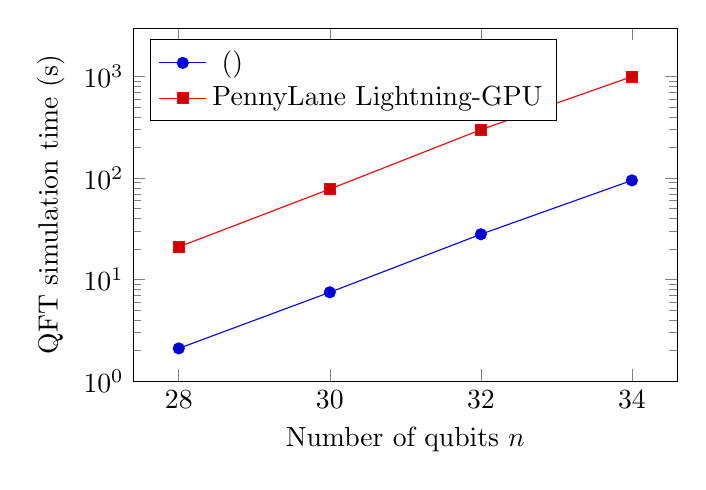
\begin{tikzpicture}
\begin{axis}[
  ymode=log, xlabel={Number of qubits $n$}, ylabel={QFT simulation time (s)},
  xtick={28,30,32,34}, ymin=1, ymax=3000,
  legend pos=north west, legend cell align=left,
  width=0.7\linewidth, height=0.5\linewidth]
  \addplot coordinates {(28,2.1) (30,7.5) (32,28) (34,95)};
  \addlegendentry{\qgear\ (\cudaq)}
  \addplot coordinates {(28,21) (30,78) (32,300) (34,1000)};
  \addlegendentry{PennyLane Lightning-GPU}
\end{axis}
\end{tikzpicture}
\caption{Simulation time of the Quantum Fourier transform versus qubit count for \qgear\ on \cudaq\ and for PennyLane Lightning-GPU on the same A100 hardware (one GPU up to 32 qubits, the four GPUs of one node at 34 qubits). Re-plotted from the approximately $10\times$ advantage reported in \cite{guo2025qgear}; intermediate points are illustrative.}
\label{fig:qgear:qft}
\end{figure}

The VQE benchmark shows the same effect from the perspective of a variational loop. An 18-qubit VQE instance that converged in 126 optimiser iterations to a percent error of \num{2.59e-7} in the ground-state energy ran in about \SI{4}{\second} end to end through \qgear\ in adjoint mode, compared with about \SI{10}{\minute} for the same optimisation through the CPU baseline, as reported in \cite{guo2025qgear}. Here each iteration evaluates the expectation values of all Hamiltonian terms on one state, so the adjoint mode's single-pass \texttt{observe} call replaces hundreds of separate circuit executions per iteration, and the converged energy agrees with the exact value to the stated precision, confirming that the transformation preserves the circuit semantics.

\subsection{\qcrank\ Image-Encoding Benchmarks}\label{sec:qgear:results-qcrank}

The final benchmark family targets the data-encoding circuits that recur throughout \cref{ch:qml,ch:synthesis}. \Cref{tab:qgear:qcrank} lists the four images used in \cite{guo2025qgear}, from a $64\times 80$ fingerprint with about 5,000 pixels to a $384\times 256$ zebra with about 98,000 pixels. In \qcrank\ the number of pixels is $2^{n_{a}}n_{d}$, so a given image admits several $(n_{a},n_{d})$ decompositions; the zebra image, for instance, was encoded with 13 address and 12 data qubits, with 14 and 6, and with 15 and 3. Because each pixel value is read out from the statistics of its address, the shot count scales with the number of address states, from three million shots for the fingerprint to 98 million shots for the 15-address-qubit zebra encoding. For the smaller images, the GPU pipeline delivered speed-ups approaching two orders of magnitude over the CPU baseline \cite{guo2025qgear}; for the largest shot counts the advantage narrows because sampling $10^{8}$ bit strings from a 25-qubit state is dominated by the sampling and host-transfer path rather than by the state-vector update that the GPU accelerates. This observation motivated the multi-shot sampling optimisations discussed in \cref{sec:qgear:discussion} and, more fundamentally, the shot-efficient encodings developed in \cref{ch:qml}.

\begin{table}[htbp]
\caption{\qcrank\ image-encoding benchmarks used in \cite{guo2025qgear}. An image of $2^{n_{a}}\times n_{d}$ pixels is loaded with $n_{a}$ address and $n_{d}$ data qubits; the shot budget grows with the number of address states. Data from \cite{guo2025qgear}.}
\label{tab:qgear:qcrank}
\centering\small
\begin{threeparttable}
\begin{tabular}{@{}llrccr@{}}
\toprule
Image & Resolution & Pixels & Address qubits $n_{a}$ & Data qubits $n_{d}$ & Shots \\
\midrule
Finger   & $64\times 80$   & 5,120  & 10 & 5  & 3\,M \\
Shoes    & $128\times 128$ & 16,384 & 11 & 8  & 6\,M \\
Building & $192\times 128$ & 24,576 & 12 & 6  & 12\,M \\
Zebra    & $384\times 256$ & 98,304 & 13 & 12 & 24\,M \\
         &                 &        & 14 & 6  & 49\,M \\
         &                 &        & 15 & 3  & 98\,M \\
\bottomrule
\end{tabular}
\begin{tablenotes}\footnotesize
\item GPU speed-ups over the CPU baseline approach two orders of magnitude for the smaller images \cite{guo2025qgear}.
\end{tablenotes}
\end{threeparttable}
\end{table}

\section{Discussion and Limitations}\label{sec:qgear:discussion}

The results above answer the first half of RQ1 quantitatively: with the GPUs available on a leadership-class system today, exact state-vector simulation reaches 42 qubits, and the 30--34-qubit regime that used to require a day of CPU time is now interactive. The second half of RQ1, usability, is answered by the design: no circuit in this chapter was rewritten, and the same HDF5 batch was executed on one GPU and on 1,024 GPUs by changing two lines of a job script. Several limitations, however, bound what this approach can deliver, and we state them explicitly because they shape the rest of the dissertation.

\emph{The memory wall.} Index-bit partitioning trades memory for GPUs at a fixed exchange rate of one qubit per doubling of the GPU count. With \SI{40}{\giga\byte} per GPU the 1,024 GPUs used here hold 42 qubits; the \SI{80}{\giga\byte} A100 and the newer H100 add one qubit, and the entire Perlmutter GPU partition of roughly 7,000 GPUs would add two or three more. Exact simulation of general circuits therefore ends at about 42--45 qubits on any machine that exists or is planned, regardless of software quality. Beyond that scale, only approximate methods such as matrix-product states \cite{perezgarcia2006mps} for low-entanglement circuits, or the circuit-cutting techniques of \cref{sec:bg:cutting}, can extend simulation, and only by exploiting structure that random circuits do not have. This is the boundary at which the hardware experiments of \cref{ch:nisq,ch:qml} become the only way to obtain answers, and it is why \qgear\ is positioned as a verification and calibration tool for circuits that are then run on QPUs, not as a replacement for them.

\emph{Communication for high-order qubits.} Along the memory-limited diagonal of \cref{fig:qgear:scaling} the time per gate rises with $n$ because the fraction of gates that touch global qubits grows with $g=n-32$ and each such gate moves half of the distributed state across the network. For random circuits the effect is mild, since global qubits are a small minority, but for structured circuits in which a few qubits are addressed by many gates, as in the QFT or in the address register of \qcrank, a fixed qubit ordering can place a heavily used qubit among the global ones and incur an exchange at nearly every layer. Choosing the permutation of logical to index bits so that the most frequently addressed qubits are local, in the spirit of the qubit-reordering strategies in \cite{bayraktar2023cuquantum,doi2023multishotgpu}, is a natural extension that the current \qgear\ release leaves to the \cudaq\ runtime.

\emph{Gate-set coverage.} The eight instructions in \cref{tab:qgear:gates} cover the workloads in this dissertation but not, for example, multi-controlled gates, arbitrary unitaries given as matrices, mid-circuit measurement with feed-forward, or reset. Some of these are straightforward additions to the dispatch table; mid-circuit measurement with classical control is not, because it breaks the pure state-vector model on which the multi-GPU partitioning relies and would require the sampling path of the simulator rather than the state-vector path. The \qawa\ circuits of \cref{ch:nisq}, which use mid-circuit measurement data, were therefore validated with \qgear\ only up to the measurement layer.

\emph{Sampling-dominated workloads.} The \qcrank\ results show that when a circuit is shallow and the shot count is in the tens of millions, the cost is dominated by sampling bit strings from the final state and transferring them to the host, a step that GPU state-vector acceleration does not address. Techniques that sample many shots from a single stored state without re-simulating the circuit \cite{doi2023multishotgpu} mitigate this, and \qgear\ uses \cudaq's multi-shot sampling, but the more fundamental remedy is to design encodings that need fewer shots, which is the subject of \cref{ch:qml}.

\emph{Precision.} All results use single-precision complex amplitudes, which halves memory relative to double precision and is what allows 32 qubits per GPU. For the circuit depths considered here the accumulated rounding error is far below the shot noise of any realistic experiment, and the VQE benchmark converged to a relative error of $10^{-7}$; for much deeper circuits, or for computing small differences of amplitudes, a double-precision target with 31 qubits per GPU is available at twice the memory cost.

\section{Relation to the Other Chapters}\label{sec:qgear:relation}

\qgear\ is the simulation substrate on which the rest of this dissertation stands, and the connection is concrete rather than rhetorical. The 20-qubit, 10-layer \deal\ circuits of \cref{ch:nisq} were simulated noiselessly through \qgear\ before submission to the IBM Torino and Marrakesh processors, both to confirm that the directly initialised angles reproduced the intended energies and to obtain the noiseless reference distributions against which the hardware success probabilities and Kullback--Leibler divergences are measured; the \qawa\ walk circuits of the same chapter were simulated up to 20 qubits with the same pipeline. In \cref{ch:qml} the \shardq\ circuit-cutting framework knits sub-circuit results on A100 GPUs, and its quasi-probability reconstruction, whose cost grows as $3^{2k}$ in the number of cuts $k$, was made tractable by running the sub-circuit simulations through the parallel mode of \cref{sec:qgear:modes}; the \qcrank\ encoders benchmarked in \cref{tab:qgear:qcrank} are the same encoders that \shardq\ cuts and that \vqt\ uses for its vectorised attention. In \cref{ch:synthesis} the \rubriq\ reinforcement-learning loop evaluates the fidelity component of its rubric reward by simulating every generated circuit in \cudaq; the constant-time kernel construction and the container deployment developed here are what make it possible to evaluate thousands of candidate circuits per training step on the same Perlmutter nodes that host the language model. Finally, the memory wall quantified in \cref{sec:qgear:discussion} is the reason the dissertation turns, in its later chapters, from simulating quantum computation to trusting it: once circuits exceed what any classical machine can check, the questions of \cref{ch:qec} about auditable error correction on shared hardware become unavoidable.

\section{Summary}\label{sec:qgear:summary}

This chapter presented \qgear, a framework that makes GPU-accelerated state-vector simulation available to \qiskit\ users without rewriting their circuits. Its three-tensor encoding with HDF5 storage decouples circuit generation from execution; its constant-time kernel transformation covers a compact but universal gate set; its adjoint and parallel modes match the two shapes of quantum workloads on an HPC system; and its containerised, Slurm-integrated deployment partitions a single state vector across GPUs by index-bit decomposition, so that the same job script runs on one GPU or on 1,024. Experiments reported in \cite{guo2025qgear} showed roughly two orders of magnitude speed-up over a 128-core CPU node, with a 34-qubit random unitary reduced from about a day to about a minute on one GPU node; roughly one order of magnitude over existing GPU simulators, with 20--100$\times$ gains on the QFT; an 18-qubit VQE reduced from ten minutes to four seconds; and exact simulation of 42-qubit circuits on 1,024 A100 GPUs at near-full utilisation. The chapter also identified the limits of the approach: a memory wall at about 42--45 qubits, communication costs for heavily used global qubits, a restricted gate set, and sampling-dominated encoding workloads. These limits motivate the hardware-aware algorithms of \cref{ch:nisq}, the shot-efficient encodings of \cref{ch:qml}, and the verification questions of \cref{ch:qec}, while the pipeline itself remains the tool with which every circuit in those chapters was first validated.
